\documentclass[10pt,letterpaper]{article}
\usepackage[letterpaper,hmargin=1.0in,vmargin=0.9in]{geometry}
\linespread{1.04}
\usepackage[T1]{fontenc}
\usepackage{XCharter}
\usepackage{fontspec}
\setmonofont{FiraMono-Regular.otf}[Scale=0.82]
\usepackage{microtype}
\usepackage{booktabs,array,tabularx}
\usepackage{graphicx}
\usepackage{float}
\usepackage[font=small,labelfont=bf,skip=6pt]{caption}
\usepackage{enumitem}
\usepackage{xcolor}
\usepackage{titlesec}
\usepackage[most]{tcolorbox}
\usepackage[hidelinks]{hyperref}

\definecolor{ink}{HTML}{0B0B0B}
\definecolor{soft}{HTML}{52514E}
\definecolor{rule}{HTML}{C3C2B7}
\definecolor{boxback}{HTML}{F4F3EE}

\setlength{\parindent}{0pt}
\setlength{\parskip}{6pt plus 1pt minus 1pt}
\setlist{itemsep=2pt,topsep=3pt,parsep=2pt,leftmargin=1.4em}
\titleformat{\section}{\large\bfseries}{\thesection}{0.6em}{}
\titlespacing*{\section}{0pt}{14pt plus 2pt minus 2pt}{4pt}
\renewcommand{\arraystretch}{1.15}
\newcommand{\s}[1]{\texttt{#1}}          % a sentence or word of the toy language
\newtcolorbox{keybox}{colback=boxback,colframe=rule,boxrule=0.5pt,arc=2pt,
  left=8pt,right=8pt,top=6pt,bottom=6pt}

\newcommand{\asof}{1:13 pm}
\newcommand{\stilltraining}{4}

\newcommand{\reads}[2]{\textbf{How to read figure \ref{#1}.} #2}
\newcommand{\shows}[1]{\textbf{What figure \ref{#1} shows.}}

\begin{document}

\begin{center}
{\LARGE\bfseries What happened next, in pictures}\\[5pt]
{\large Third report on the vocabulary experiment, 22 November 2026}\\[3pt]
{\small\color{soft} Prepared by Claude. The pictures show the runs as they ended, or were stopped, on 22 November.}
\end{center}

\begin{keybox}
\textbf{What this report holds.} The first report covered the night's experiment, and the
addendum covered the yes-or-no questions. This report holds what is in neither of them:
\begin{enumerate}[itemsep=1pt,topsep=2pt]
\item \textbf{The 32-bit round, carried further,} as you asked: the runs that had run out of
      time were trained on, and the languages that had never been run were run, as far as the work went
      (sections \ref{sec:t32} and \ref{sec:tkinds}).
\item \textbf{Pictures of results} that so far existed only as tables, or not at all
      (sections \ref{sec:tq} to \ref{sec:ttext}).
\end{enumerate}
I have kept my own opinions out of the sections with pictures. They are in section
\ref{sec:tview}, so that you can look first and judge for yourself.

\textbf{How to read every picture.}
\begin{itemize}[itemsep=1pt,topsep=2pt]
\item Each thin line, and each dot, is one model trained once (one ``run''). The two
      exceptions, figures \ref{fig:teffort} and \ref{fig:ttext}, say so.
\item Color is the width of the model: orange is width 8, green is width 16, yellow is
      width 32. In figures \ref{fig:tba} and \ref{fig:tcourse} color is the size of the
      vocabulary instead.
\item Scores run from 0 (no better than guessing) to 100 (everything right).
\item A ``set'' is one portion of training text, the same size for every model. Where sets
      are on a scale, the scale is stretched so that equal distances mean equal multiples:
      10, 100 and 1,000 are equally far apart.
\item \stilltraining{} runs were stopped by hand while still training, and are not saved. In
      figures \ref{fig:t32} and \ref{fig:tstand} they are marked with a triangle pointing
      right. Their lines end where they were stopped.
\end{itemize}

\textbf{Words from the earlier reports.} A \emph{repeat} is the same experiment started
afresh with new starting numbers. \emph{Equal use} means every animal is mentioned equally
often; \emph{unequal use} means some animals are mentioned far more often than others. The
\emph{32-bit round} is the one in which each animal has 16 facts, its four facts for each of
four seasons. The \emph{stopping test} is the rule of the first night that ended a run when
its score had stopped rising.
\end{keybox}

\section{The 32-bit round, carried further}\label{sec:t32}

In the 32-bit round each animal has 16 facts: its four facts for each of four seasons. When the
first report was written, this round stood as follows. On 16 animals every width had learned
every statement. On 256 animals widths 16 and 32 had learned them and width 8 had not. On 1,024
animals two runs had run out of time. The 64-animal language, and width 8 on 1,024 animals,
had never been run.

Since then, as you asked, I picked the unfinished runs up again from where they had been saved
and went on training them, and started the runs that had never been made. Each has a time
limit of 2 to 5 hours.

\clearpage
\begin{figure}[H]
\centering
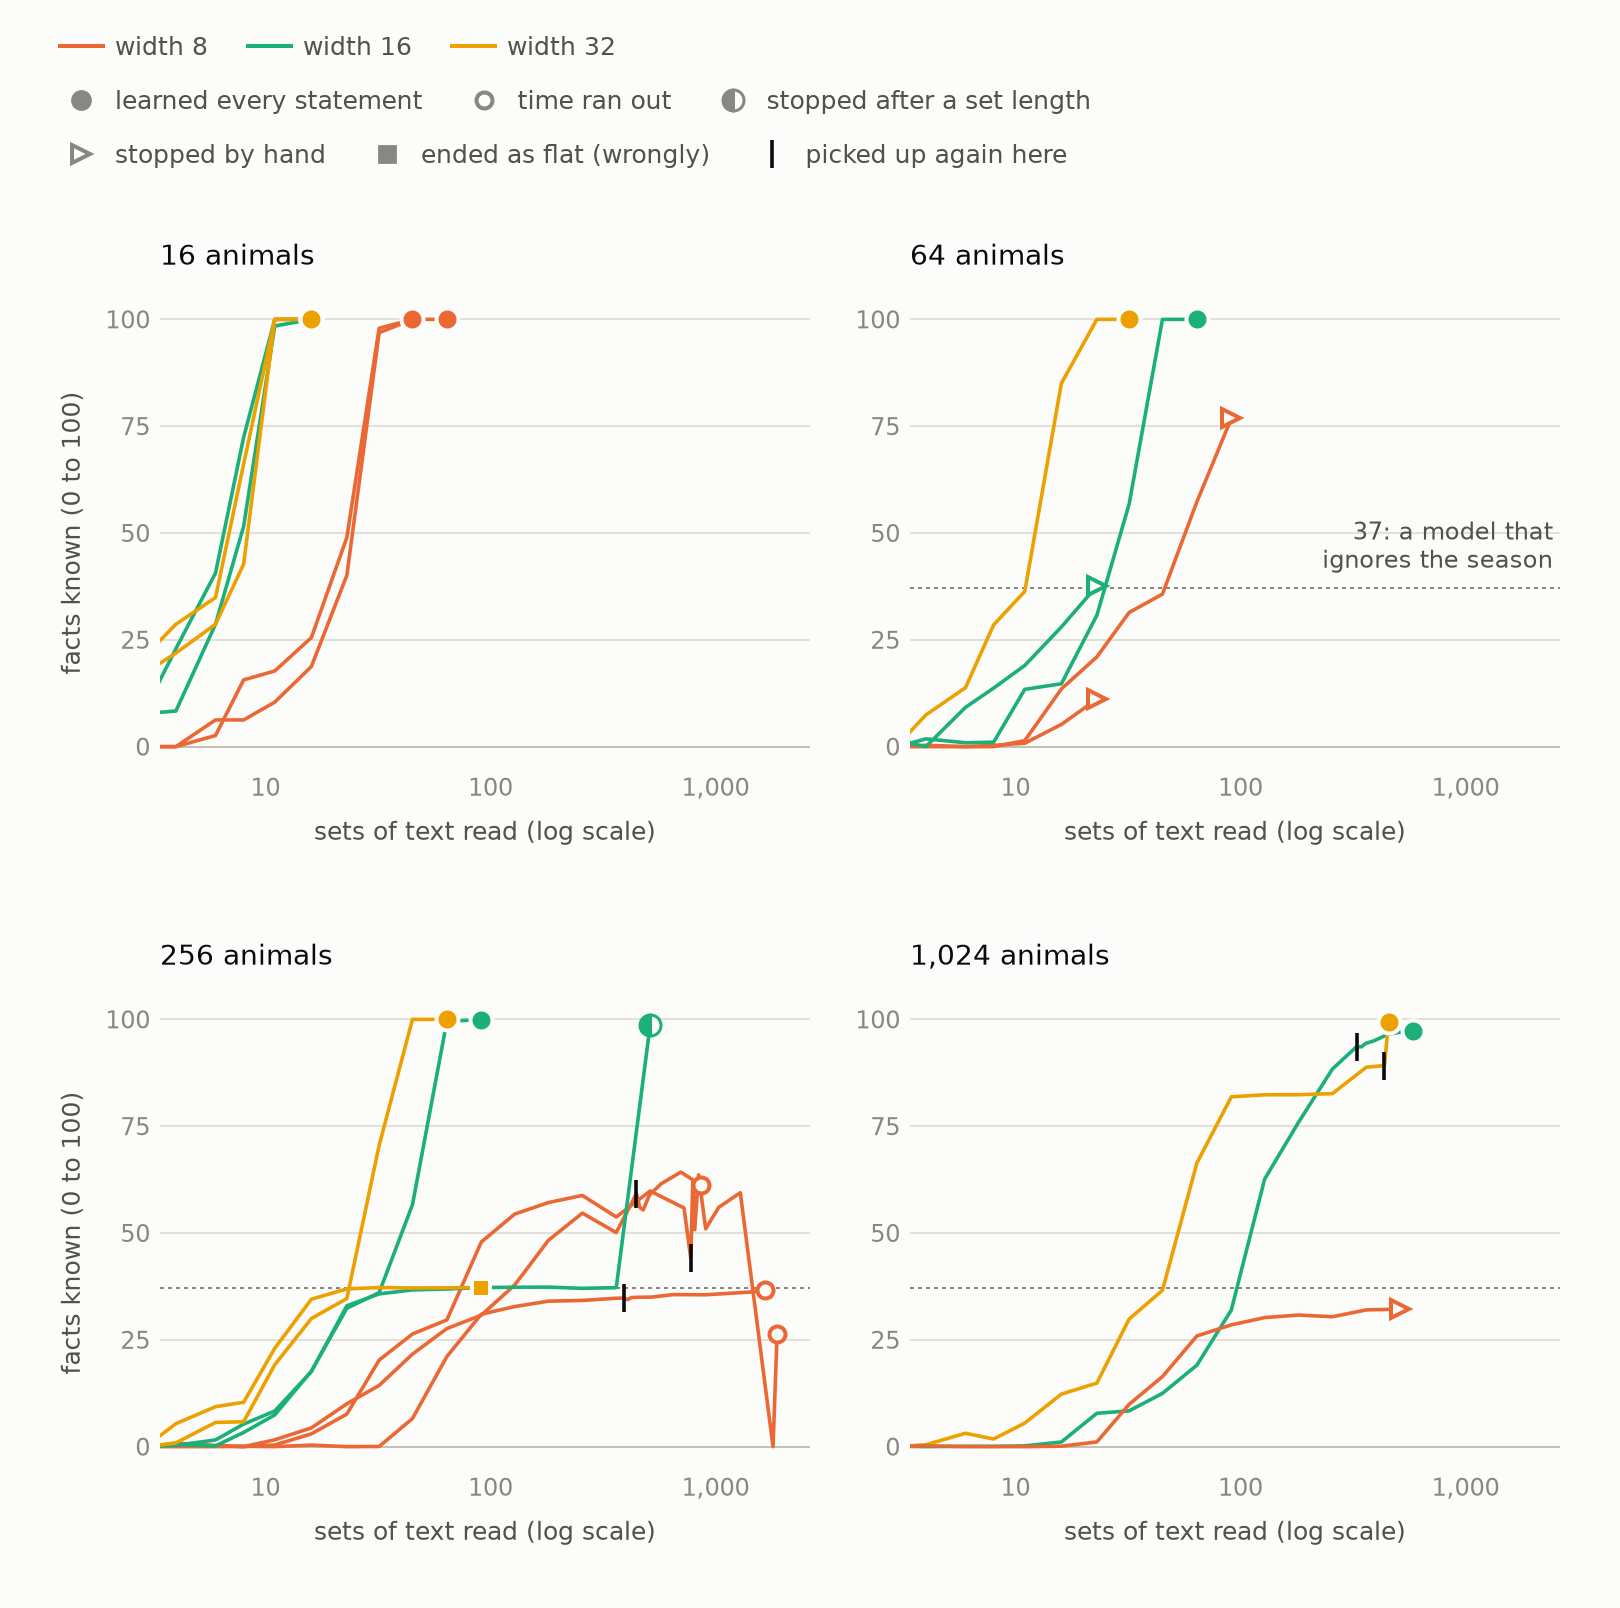
\includegraphics[width=0.84\textwidth]{figures/t_round32.png}
\caption{The 32-bit round. Each panel is one size of vocabulary, and each line is one run: how
many facts the model knew as it read more and more text.}
\label{fig:t32}
\end{figure}

\reads{fig:t32}{Follow a line from left to right: it is one model learning. A line that
reaches the top has learned every statement. The mark at the end of a line says how the run
ended. A filled dot: it learned every statement. A hollow dot: its time ran out. A half-filled
dot: it was stopped after a length fixed in advance (512 sets). A square: the stopping test
ended it as flat, wrongly as it turned out. A triangle: it was still training when I stopped it by hand. A short black
tick on a line is the place where a run that had run out of time was picked up again. The
dotted line at 37 is the score of a model that knows what each animal is usually like and
takes no notice of the season.}

\shows{fig:t32}
\begin{itemize}
\item \textbf{16 animals.} Every run of every width reaches the top within 64 sets.
\item \textbf{64 animals} (new). Width 32 reaches the top in 32 sets, without pausing at the
      dotted line. Width 16 reaches the top too (100.0). Width 8 was stopped by hand at 76.8
      after 91 sets, still rising. The second repeat was stopped at 37.6 (width 16) and 11.1
      (width 8), both after 23 sets; for width 32 it was never started.
\item \textbf{256 animals.} Widths 16 and 32 reach the top. Two of their runs first lie flat on
      the dotted line; one of those was ended there by the stopping test, and the other
      climbed after set 362. The three orange lines are width 8. Since being picked up again,
      none of them has reached the top. Their time limits ended them at 61.3 (after 413 extra
      sets), 36.6 (after 1,259 extra sets) and 26.4 (after 1,101 extra sets).
\item \textbf{1,024 animals.} Width 32, picked up again at set 436, reached the top at set 459.
      Width 16, picked up at set 328, crept from 93.6 to 97.4 after 256 extra sets, and ended
      as learned; its question score was 39.5. Width 8 (new) was stopped by hand at 32.2
      after 512 sets.
\end{itemize}

\clearpage
\begin{figure}[H]
\centering
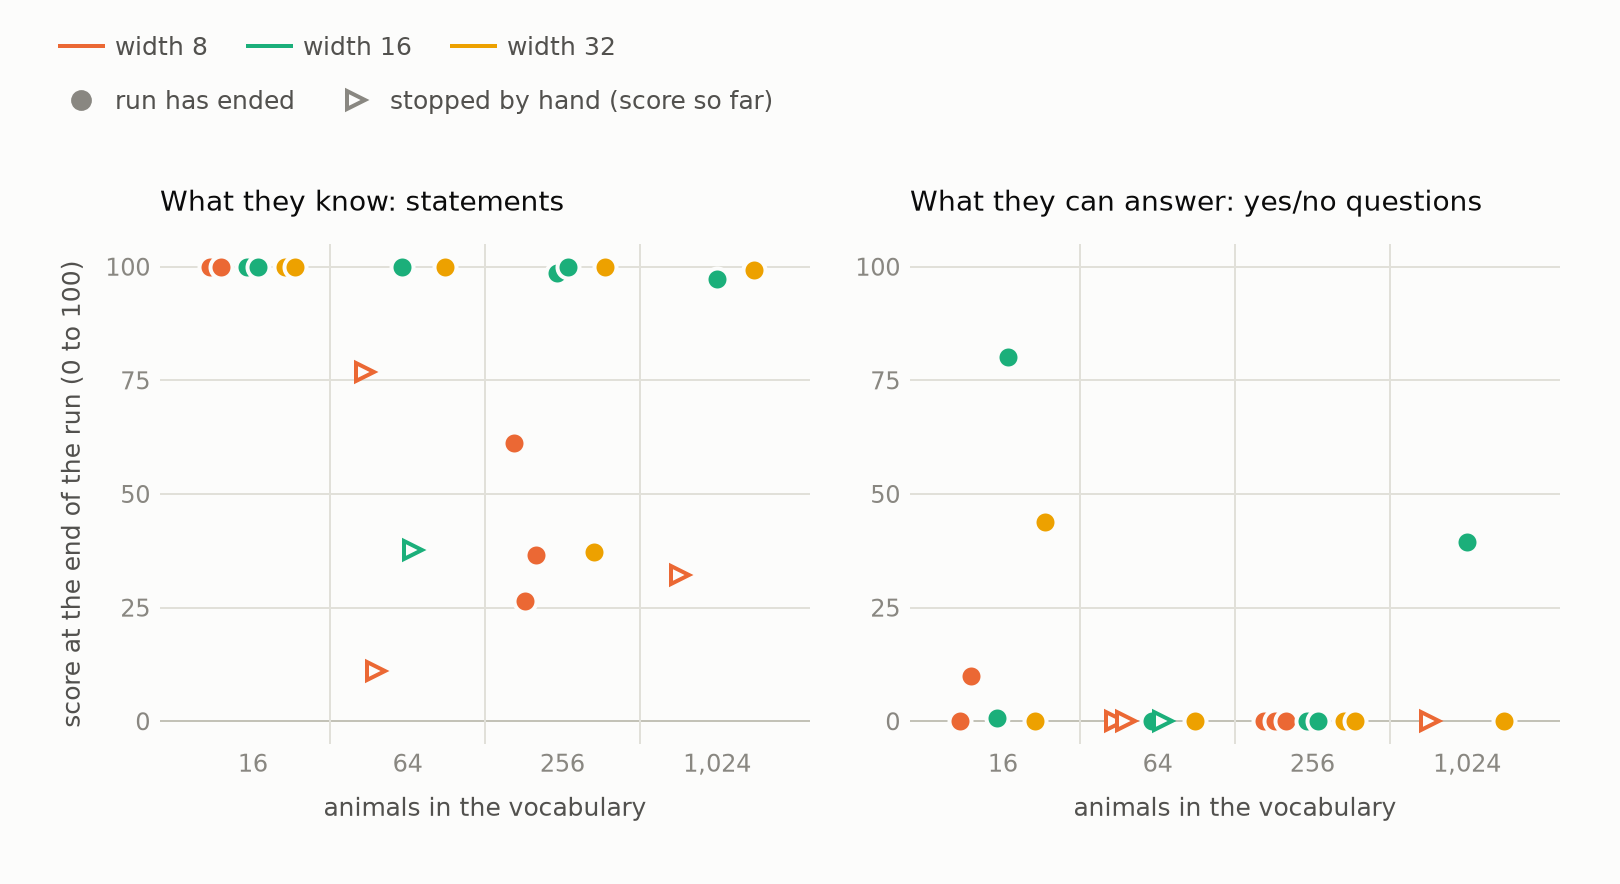
\includegraphics[width=0.95\textwidth]{figures/t_stand.png}
\caption{Where every model of the 32-bit round stands. Left: its score on the statements.
Right: its score on the yes-or-no questions about the same facts.}
\label{fig:tstand}
\end{figure}

\reads{fig:tstand}{Each dot is the latest score of one run, grouped by the size of its
vocabulary. Within a group the dots are nudged sideways, orange then green then yellow, so
that they do not hide each other. A triangle is a run that was stopped by hand while still training. Width 32 on 256
animals has two dots on the left: its first run, which the stopping test ended at 37, and the
same run made again, which reached 100.}

\shows{fig:tstand}
\begin{itemize}
\item \textbf{Left.} Most models are at or near 100 on the statements. The ones well below are
      width 8 on 256 and on 1,024 animals, the width 8 runs on 64 animals that were stopped by
      hand, and the one run that was ended at 37.
\item \textbf{Right.} Almost all of the same models are at 0 on the questions. Only a few of
      the 16-animal models, and width 16 on 1,024 animals, are above it.
\end{itemize}

\clearpage
\section{Width 8 on 256 animals, one kind of fact at a time}\label{sec:tkinds}

Width 8 on 256 animals is the case that the first report called the nearest thing to your
prediction. The statement score counts all facts together. This picture splits it into the
four kinds of fact.

\begin{figure}[H]
\centering
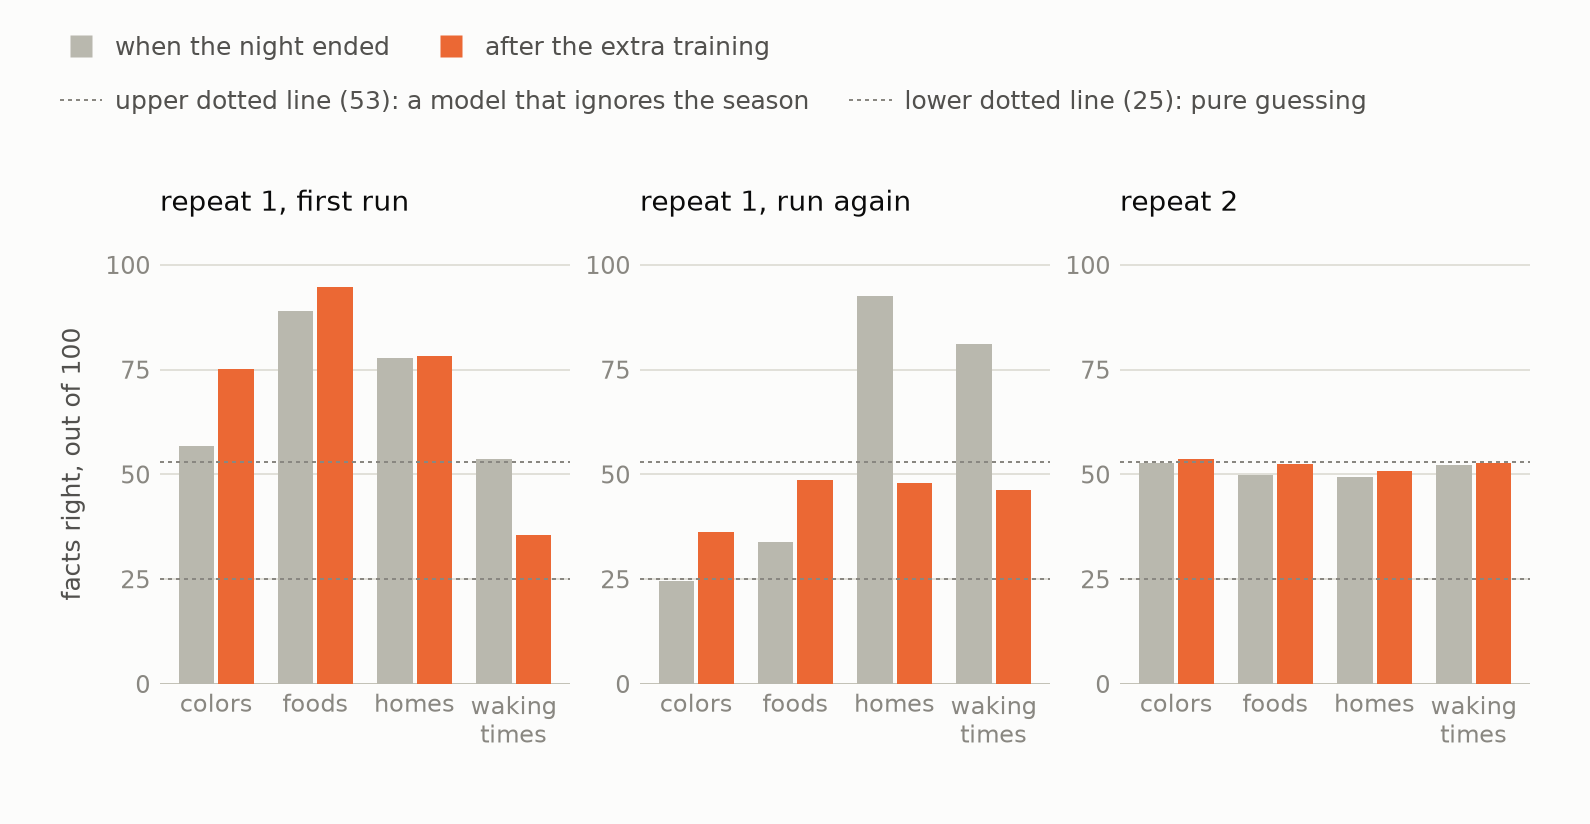
\includegraphics[width=0.9\textwidth]{figures/t_kinds.png}
\caption{Width 8 on 256 animals with 32 bits each: how many facts of each kind its three runs
had right, out of 100: when the night ended (gray) and after the extra training (orange).}
\label{fig:tkinds}
\end{figure}

\reads{fig:tkinds}{Each panel is one run, and each pair of bars is one kind of fact: gray is
when the night ended, orange is after the extra training. A bar at 100
would mean every fact of that kind right. The upper dotted line, 53, is where a model stands
that ignores the season. (That is the same model as the dotted line at 37 in figure
\ref{fig:t32}: 53 facts right in 100 is a score of 37, because the score counts the 25 in 100
that guessing gives as zero.) The lower dotted line, 25, is pure guessing among the four
values.}

\shows{fig:tkinds}
\begin{itemize}
\item \textbf{First run of the first repeat:} when the night ended, foods and homes were high
      and colors and waking times were near the upper dotted line. After the extra training,
      colors rose from 57 to 75 and foods from 89 to 95, homes stayed at 78, and waking times
      fell from 54 to 36.
\item \textbf{The same start, run again:} homes and waking times were high (93 and 81), foods
      low (34) and colors at pure guessing (25). After the extra training the four kinds are all
      between 36 and 49: homes and waking times fell, colors and foods rose.
\item \textbf{Second repeat:} all four kinds were at the upper dotted line, and after the
      extra training they still are (51 to 54).
\end{itemize}

\clearpage
\section{The questions, before and after more training}\label{sec:tq}

The addendum gave these results as tables. This is the same data as a picture, for the 72
models of the two planned rounds.

\begin{figure}[H]
\centering
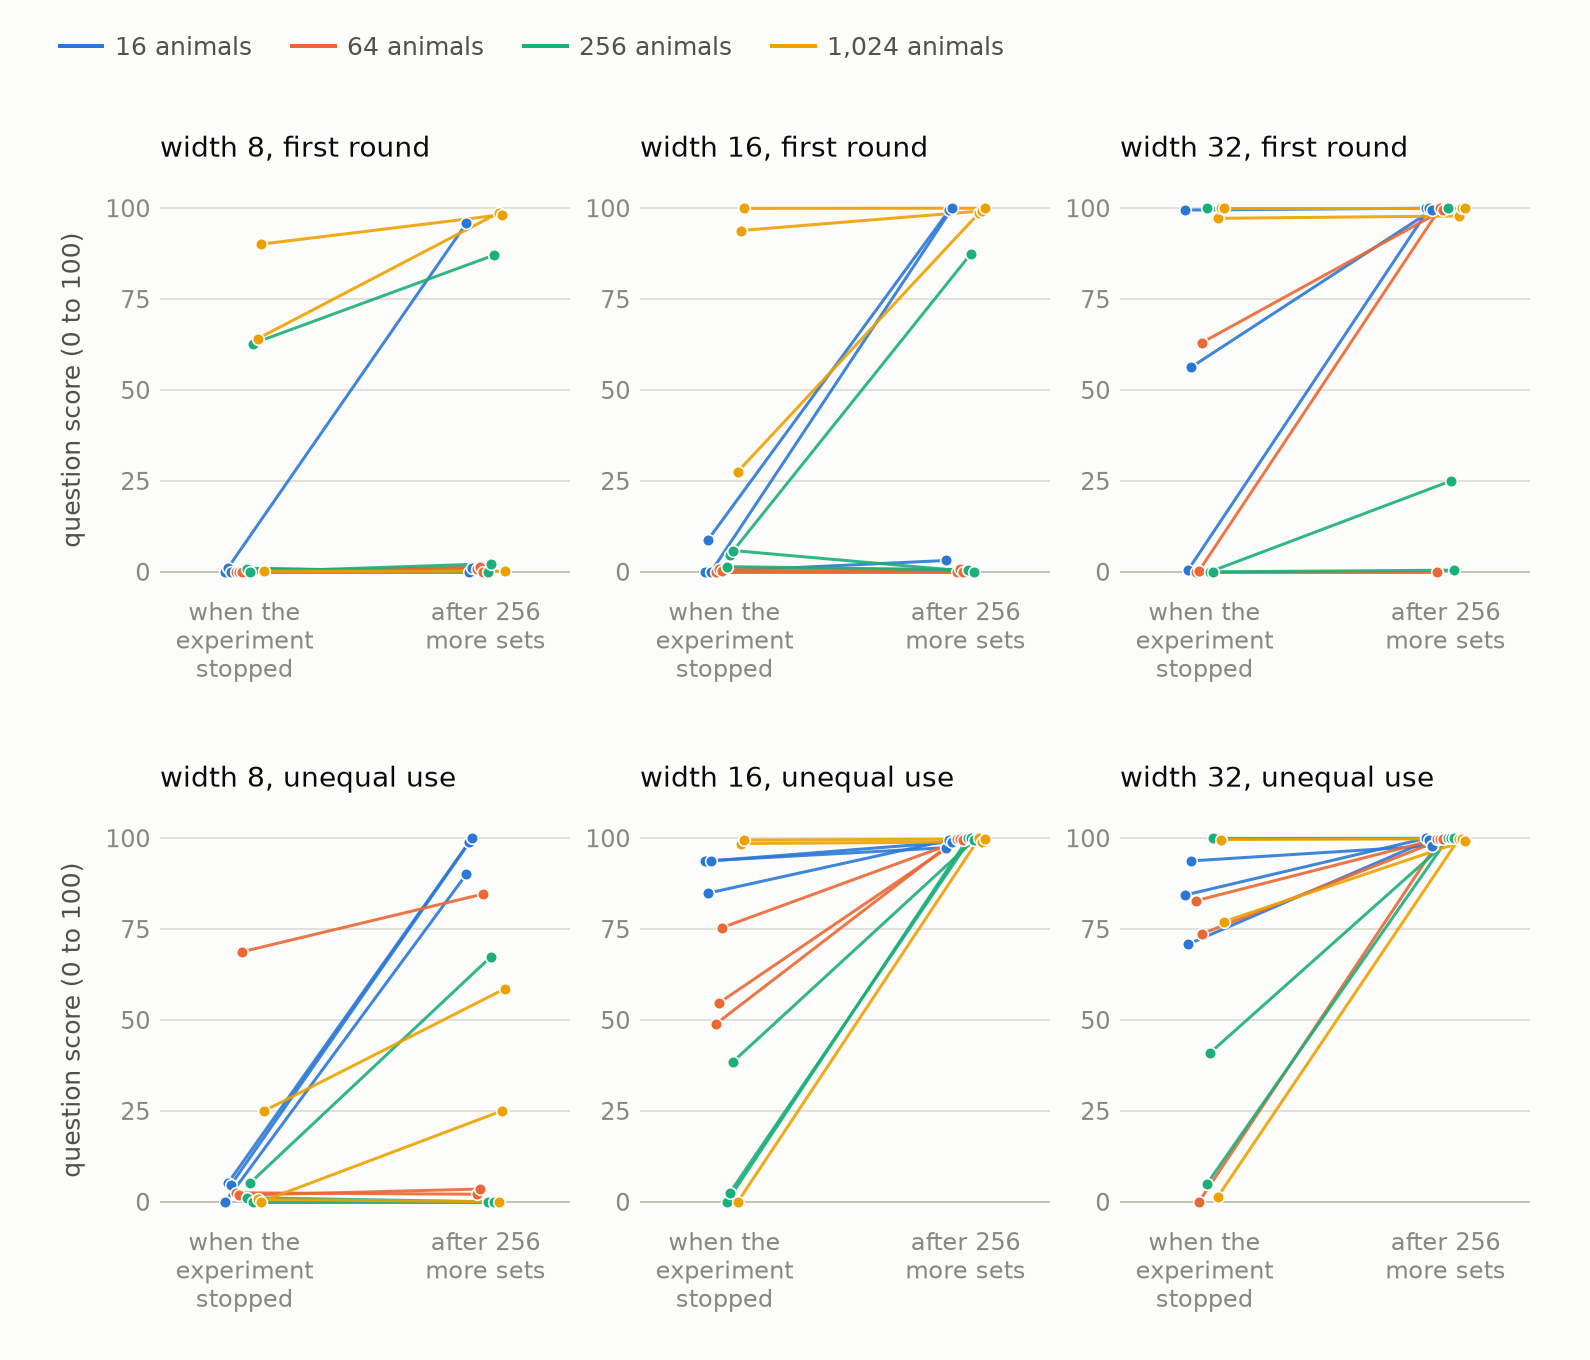
\includegraphics[width=0.9\textwidth]{figures/t_before_after.png}
\caption{The question score of every model before and after 256 more sets of training. In
this picture color is the size of the vocabulary.}
\label{fig:tba}
\end{figure}

\reads{fig:tba}{Each line is one model; each panel has 12 of them (four sizes of vocabulary,
three repeats each). The left end of a line is the model's question score when the experiment
stopped it, and the right end is its score after 256 more sets of the same text. A line that
rises learned the questions; a line along the bottom did not. The top row of panels is the
first round (equal use), the bottom row is unequal use; the columns are the three widths.}

\shows{fig:tba}
\begin{itemize}
\item \textbf{Width 32} (right column): nearly every line ends at the top. With equal use two
      lines stay at the bottom and one reaches 25.
\item \textbf{Width 16} (middle): with unequal use every line ends at the top. With equal use
      six lines stay at the bottom.
\item \textbf{Width 8} (left): with equal use most lines stay at the bottom. With unequal use
      the three blue lines (16 animals) reach the top, and some of the others rise part of
      the way.
\item Counting a question score of 90 or more as answering well, the models that answer well
      went from 8 to 17 of 36 with equal use, and from 7 to 27 of 36 with unequal use.
\end{itemize}

\clearpage
\section{Which came first, the statements or the questions?}

\begin{figure}[H]
\centering
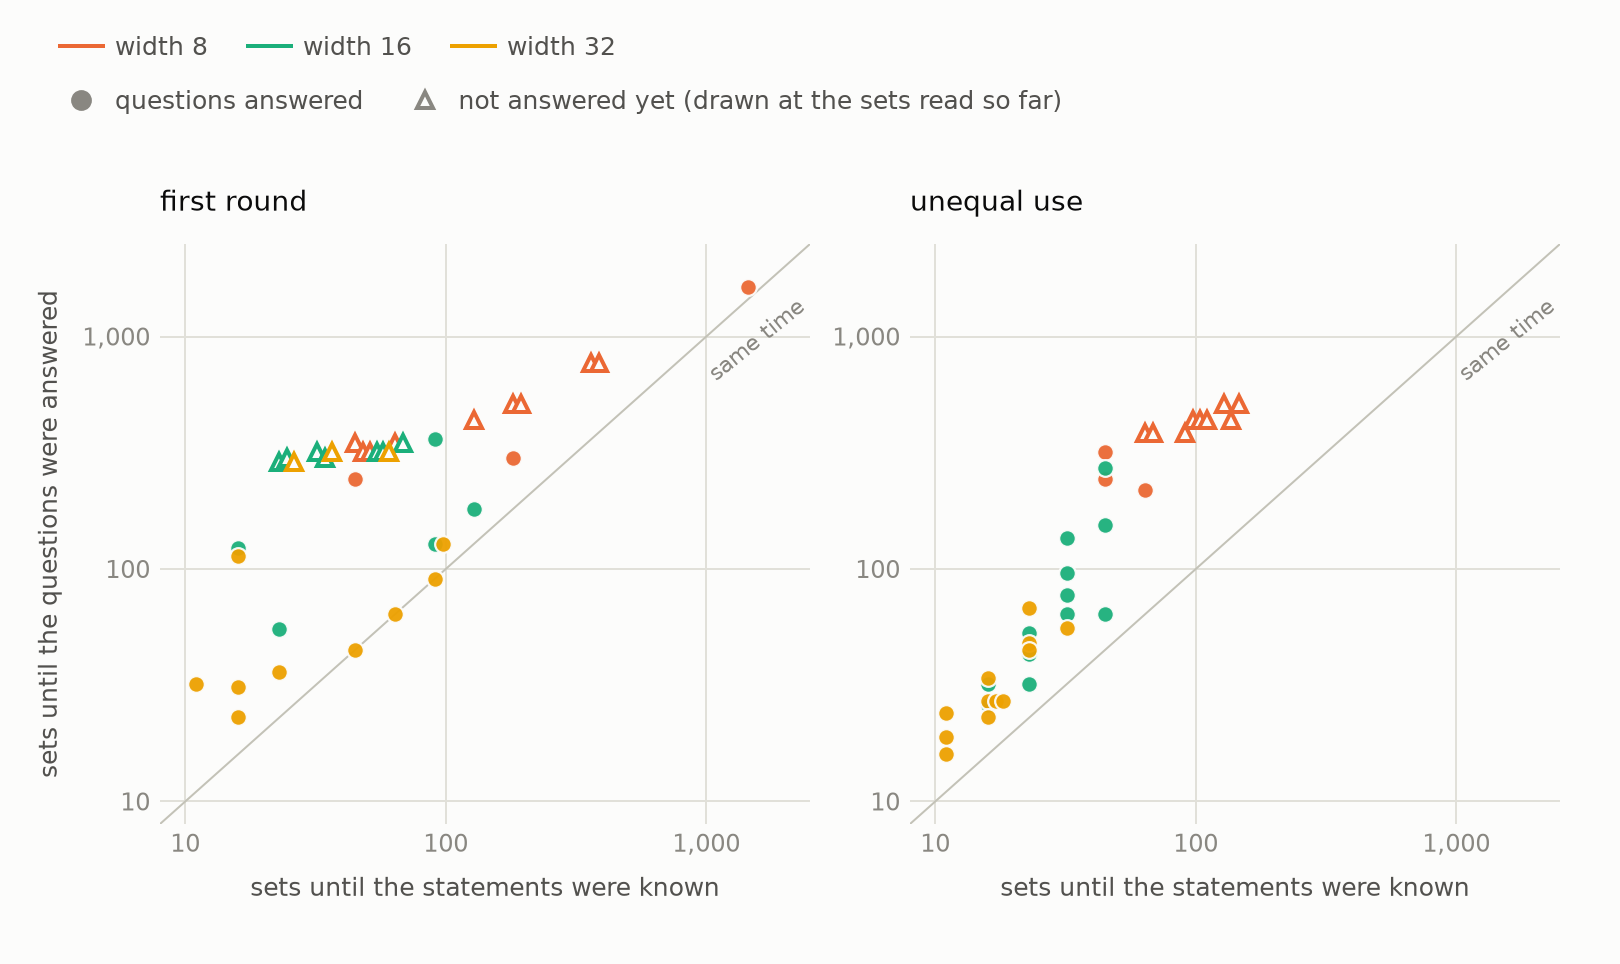
\includegraphics[width=\textwidth]{figures/t_when.png}
\caption{For each model of the two planned rounds: how many sets it had read when it knew
the statements, and how many when it could answer the questions.}
\label{fig:twhen}
\end{figure}

\reads{fig:twhen}{Each mark is one model. The further right, the longer it took to learn
the statements. The higher, the longer it took to learn the questions. A mark on the slanted
line learned both at the same time, and a mark above the line learned the questions later;
one grid line above the slanted line means ten times as long. A hollow triangle pointing up is
a model that still cannot answer the questions. It is drawn at the number of sets it has read
so far, so its true place is somewhere higher.}

\shows{fig:twhen}
\begin{itemize}
\item No mark is below the line: no model learned the questions before the statements.
\item Yellow marks (width 32) lie closest to the line, and orange marks (width 8) furthest
      above it.
\item In the first round the hollow triangles are of all three colors (9 orange, 7 green, 3
      yellow). With unequal use all 9 are orange.
\item Where a model did learn the questions, it needed between 1 and 8 times as many sets as
      for the statements; the middle value is about 2.
\end{itemize}

\clearpage
\section{The question score through the whole of training, with unequal use}

The addendum showed this picture for the first round only. Here is the unequal-use round.

\begin{figure}[H]
\centering
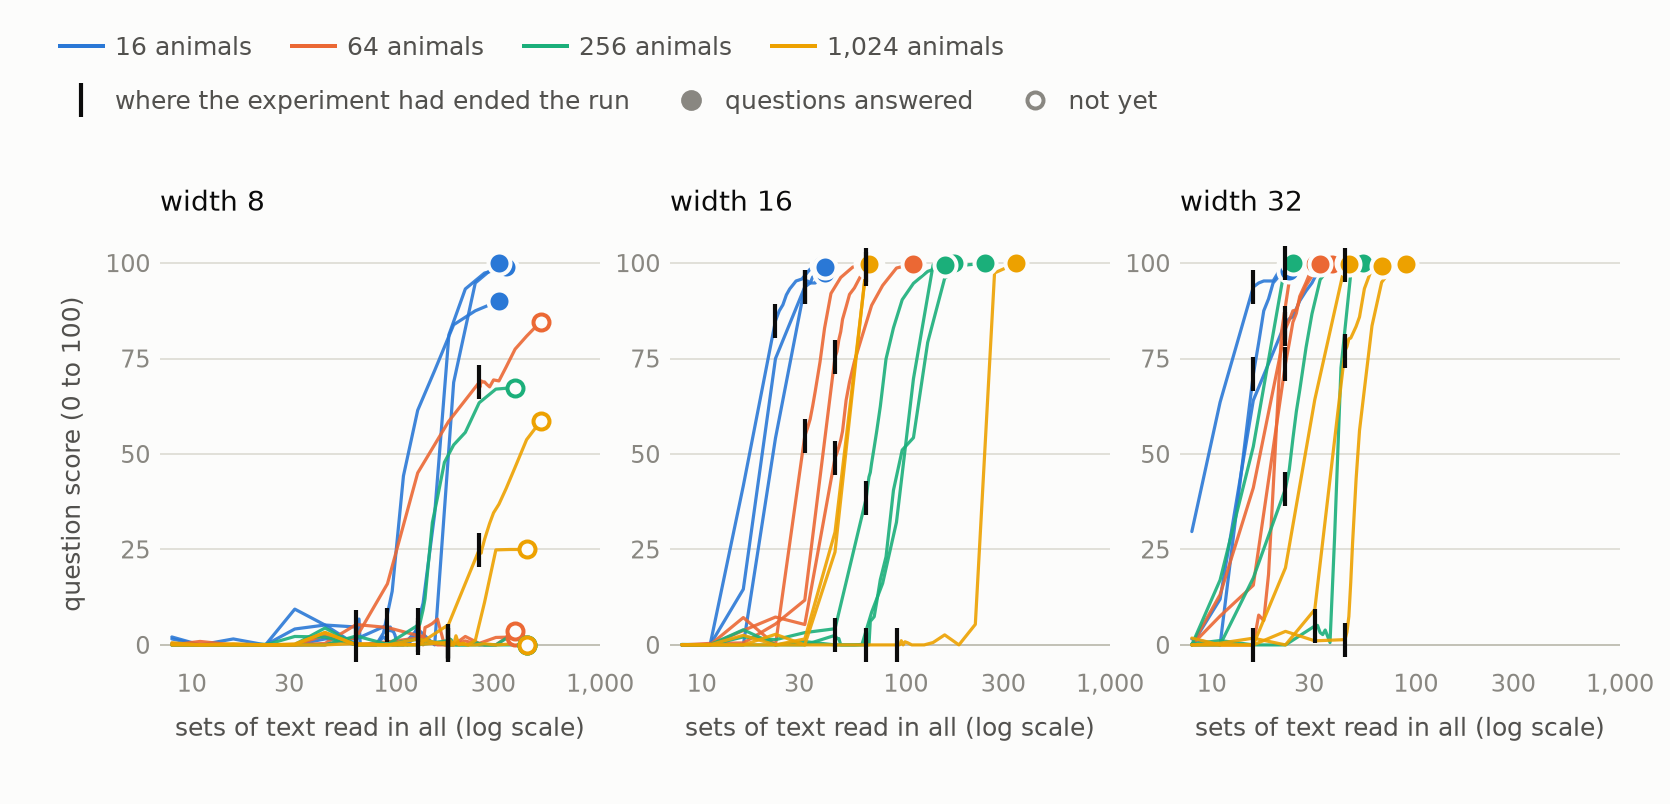
\includegraphics[width=\textwidth]{figures/t_course_zipf.png}
\caption{Unequal use. The question score of each model against all the sets it has read: its
original run, then the extra training. In this picture color is the size of the vocabulary.}
\label{fig:tcourse}
\end{figure}

\reads{fig:tcourse}{Each line is one model's question score as it reads more text. The black
tick on each line is where the experiment had ended the run; everything to the right of the
tick is the extra training. A filled dot at the end is a model that answers the questions; a
hollow dot is one that does not yet.}

\shows{fig:tcourse}
\begin{itemize}
\item At widths 16 and 32 every line ends at the top. Those that were not there yet at their
      tick climb steeply soon after it.
\item At width 8 the three blue lines (16 animals) climb to the top; the others rise part of
      the way or stay on the floor.
\end{itemize}

\clearpage
\section{More words, more text: the statements}

These are results of the first night, for the two rounds in which each animal has four facts.
The first report gave them as a table of numbers; the pictures were left out for lack of room.

\begin{figure}[H]
\centering
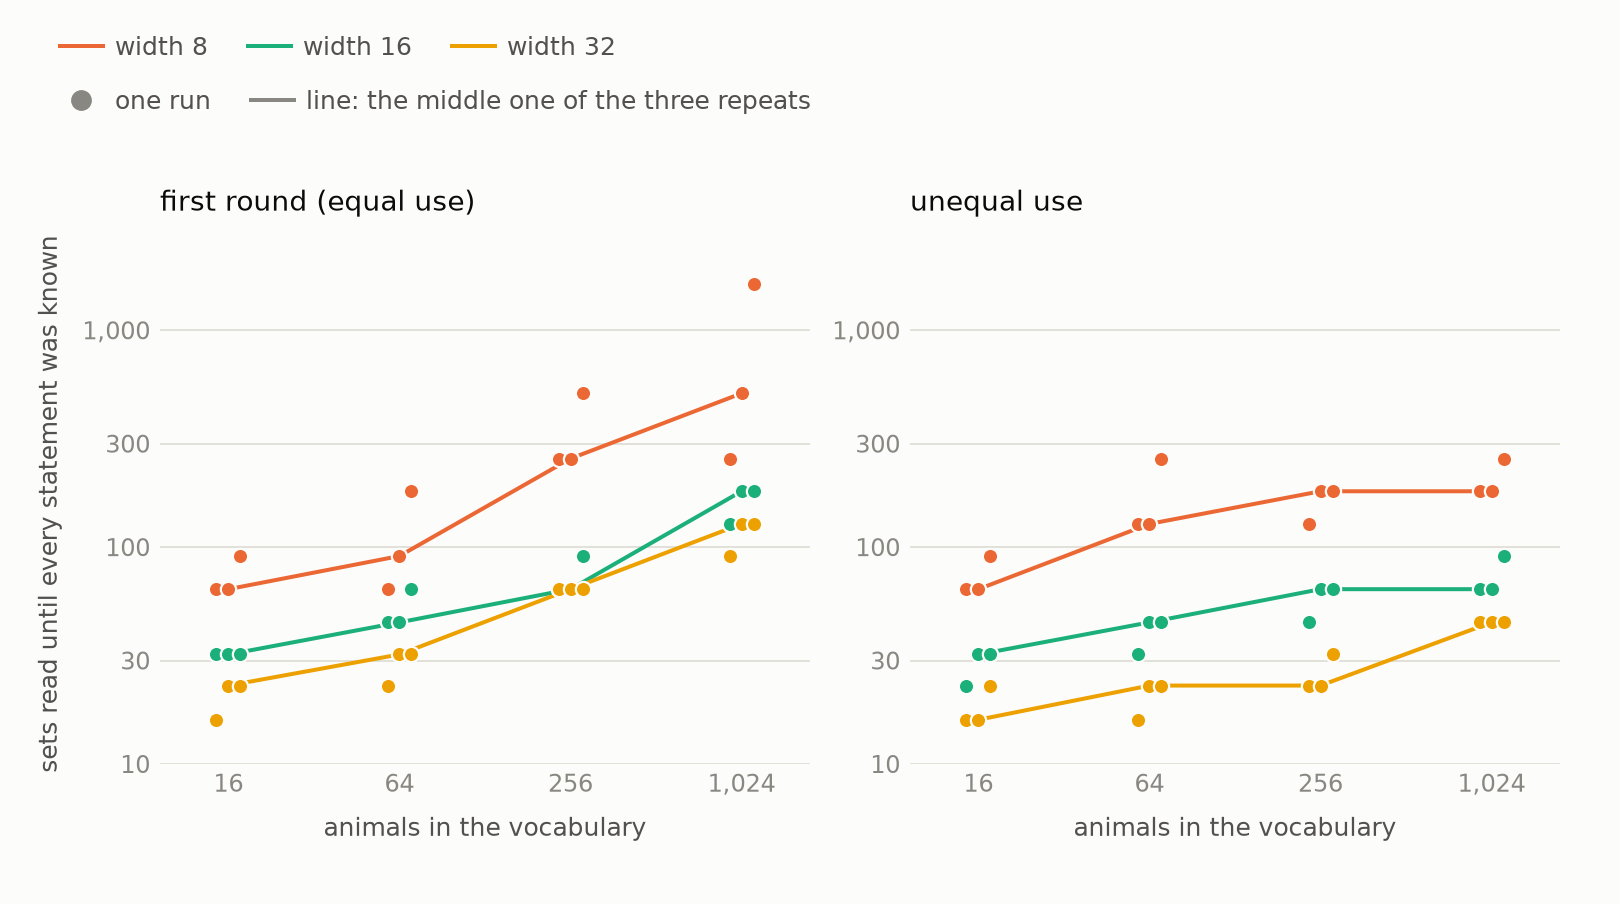
\includegraphics[width=\textwidth]{figures/t_effort.png}
\caption{How many sets each model had read when it knew every statement, against the size of
its vocabulary. Both panels use the same scale.}
\label{fig:teffort}
\end{figure}

\reads{fig:teffort}{Each dot is one run, placed above the size of its vocabulary; the higher
the dot, the more text the model needed. The three dots of a group are the three repeats. The
line is not a model: it joins the middle one of the three repeats, to show the trend.}

\shows{fig:teffort}
\begin{itemize}
\item No line falls to the right: more animals took as many sets or more.
\item The orange line (width 8) is the highest in both panels, and its dots are the most
      scattered.
\item With unequal use the right-hand ends are much lower. On 1,024 animals the middle run
      needed 181, 64 and 45 sets at widths 8, 16 and 32, against 512, 181 and 128 with equal
      use. On the smaller vocabularies the two panels are close.
\end{itemize}

\clearpage
\section{How much variety the text has}\label{sec:ttext}

You asked whether each set holds new sentences. It does not, and this picture shows how
little variety the smaller languages have.

\begin{figure}[H]
\centering
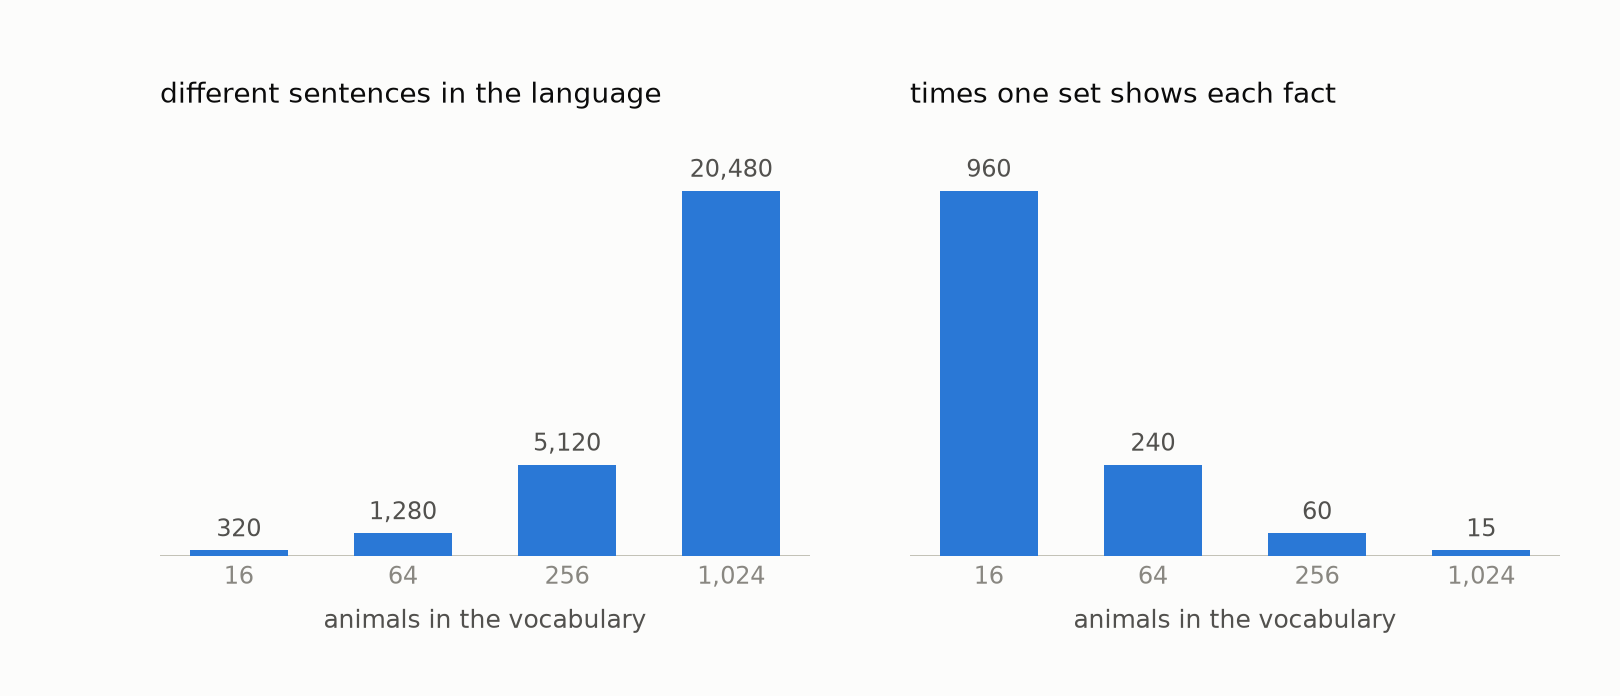
\includegraphics[width=0.66\textwidth]{figures/t_text.png}
\caption{Left: how many different sentences each language has. Right: how many times one set
of text shows each fact (first round).}
\label{fig:ttext}
\end{figure}

\reads{fig:ttext}{Each bar is one size of vocabulary; the bars here are counts, not models.
A fact (say, what foxes eat) is told by several different sentences: one statement and four
questions. Every set has the same number of sentences, 61,440, whatever the language.}

\shows{fig:ttext}
\begin{itemize}
\item The 16-animal language has only 320 different sentences. Its 64 facts are each shown
      960 times in one set (64 times 960 is the 61,440 sentences of a set).
\item The 1,024-animal language has 20,480 different sentences. Its 4,096 facts are each
      shown 15 times in one set.
\end{itemize}

\section{Also since the first report, without pictures}

\textbf{The review of the research that you asked for.} A subagent looked for what is known
about models that stand still for a long time and then jump. The full text, with 31 sources,
is in \s{results/literature\_stalls.md}. In short: researchers call it a loss plateau followed
by abrupt learning. The remedies it ranked highest for this experiment are, in order:
reshaping the text (unequal use, or starting on a few animals), sharpening the model's
attention, larger starting numbers, and running several repeats. None of them has been tried
here yet, and nearly all the evidence comes from far larger models.

\textbf{How long width 8 took.} Everything width 8 finished took about 1 hour 40 minutes of
training in all: 65 minutes for the 12 runs of the first round, 28 minutes for the 12 runs
with unequal use, and 9 minutes for the two runs on 16 animals in the 32-bit round. Its runs
on 256 animals in the 32-bit round took a further 6 and a half hours during the night without
finishing. They were then picked up again, and ended by their time limits without learning.

\section{My own reading}\label{sec:tview}

You asked to judge for yourself, so this is short, and you can skip it.
\begin{itemize}
\item \textbf{Width is the most consistent thing in every picture.} Wider models are faster on
      the statements, they learn the questions sooner and more often, and width 8 is the one
      that stays low on the larger 32-bit languages.
\item \textbf{Width 8 on 256 animals looks more and more like a model that is too small,} not
      one that is slow. Picked up again and given hours more, its three runs ended at 61.3,
      36.6 and 26.4, and none learned the statements. The picture by kind of fact shows each
      holding about two of the four kinds at a time, or fewer. This is a reading of three runs, and
      I cannot rule out that longer training would have helped.
\item \textbf{More words did not make the wider models fail.} Width 32 learned 1,024 animals
      with 32 bits each (99.4, at 459 sets in all), the largest language of the whole
      experiment. Width 16 learned it too (97.4, after 256 extra sets).
\item \textbf{Width 8 on 1,024 animals and on 64 animals is not settled.} Both runs were
      stopped while still rising (32.2 at 512 sets; 76.8 at 91 sets), so I do not know where
      they would have ended.
\item \textbf{Knowing a fact and answering a question about it are separate,} in every round.
      On 1,024 animals width 16 knew 97.4 of the statements but scored only 39.5 on the
      questions.
\item \textbf{Unequal use helps everything it touches,} which fits the first remedy of the
      research review.
\end{itemize}

\textbf{A limit of every comparison between widths, which you pointed out on 22 November.}
In this model the width is two things at once: the number of numbers in each word's row of
the word table, and the size of the body that works on those rows. Going from width 8 to 16
to 32 changed both together. So the pictures show that a wider model does better, but they
cannot show whether that comes from the longer rows or from the larger body. Comparisons
inside one width, between vocabularies, do not have this problem. I should have raised it
when the experiment was designed.

\section{How the runs ended}

Of the runs of the last batch, these ended by themselves:
\begin{itemize}
\item \textbf{Learned the statements.} 1,024 animals, width 32 (99.4, at 459 sets in all);
      1,024 animals, width 16 (97.4 after 256 extra sets); 64 animals, width 32, repeat 1 (in
      32 sets); 64 animals, width 16, repeat 1 (100.0).
\item \textbf{Ended by their time limit, not learned.} The three runs of width 8 on 256
      animals that were picked up again: 26.4 after 1,101 extra sets, 36.6 after 1,259 extra
      sets, and 61.3 after 413 extra sets.
\end{itemize}
These were stopped by hand on 22 November at about 1 pm, at your instruction, because the
work moved to a second experiment. They are not saved, and the pictures draw them from their
logs, up to where they stopped:
\begin{itemize}
\item 1,024 animals, width 8: 32.2 at 512 sets.
\item 64 animals, width 8, repeat 1: 76.8 at 91 sets.
\item 64 animals, width 16, repeat 2: 37.6 at 23 sets.
\item 64 animals, width 8, repeat 2: 11.1 at 23 sets.
\end{itemize}
One run was never started: 64 animals, width 32, repeat 2.


\end{document}
